%\documentclass{article}
%\usepackage[utf8]{inputenc}

\documentclass[12pt]{article}
\usepackage{graphicx} % This lets you include figures
\usepackage{hyperref} % This lets you make links to web locations
\graphicspath{ {./images/} }

\usepackage[rightcaption]{sidecap}
\usepackage{subcaption}
\usepackage{wrapfig}
\usepackage{listings}

\usepackage{float}

\usepackage{imakeidx}

\makeindex


\title{Feeding Families User Manual}
\date{\today}

\begin{document}
\maketitle{}

\tableofcontents

\clearpage
\newpage

\section{Introduction} %%%%%%%%%%%%%%%%%%%%%%%%%%%%%%%%%%%%%% Section 1
\subsection{About Feeding Families}
Feeding Families is a UK non-profit organization that aims to provide food hampers to disadvantaged families, with volunteers helping to organize and distribute. This system acts as a portal, hosted separately from the main Feeding Families website so that potential volunteers are able to follow a link in order to carry out the registration process. Applicants enter their information on to the website, carry out training modules provided by the charity and carry out a quiz that will verify their knowledge on the content. 

\subsection{System Overview}
The application was built using the JavaScript runtime environment, Node JS. JavaScript, HTML, CSS and MySQL were all used to develop the website and the database. We are currently using Heroku as a cloud application hosting platform for demonstration purposes. 
If the user wants to register as a volunteer, they should click on the ‘volunteer’ button on Feeding Families’ main website. After signing up or logging in through the on the redirected portal, users will choose the type of volunteer they wish to register as and then begin filling out the respective form. The volunteer’s details and all the relevant centre information will be submitted and stored onto a MySQL database. Currently, the MySQL database is hosted on the website ‘remotemysql’ which can be changed by the charity in the future to any hosting service they choose. Users will be able to log in themselves and change any of their details. The user will then complete a a set of interactive and engaging training modules which are tailored towards the role they are applying for. After completing these modules, the user will be tasked with a quiz which reference the information that they learnt throughout the training modules. Admin users are able to create reports which allow them to export to excel.

\newpage
\section{Setup} %%%%%%%%%%%%%%%%%%%%%%%%%%%%%%%%%%%%%% Section 2



\subsection{Auth0}
This section covers how to make an Auth0 account and how to integrate the Auth0 service with the volunteer portal.

\subsubsection{Setting up an account}
Go to \href{https://auth0.com/signup}{auth0.com} and sign up to an account. One of the first pages you see after making an account will look like this:
\begin{figure}[H]
    \centering
    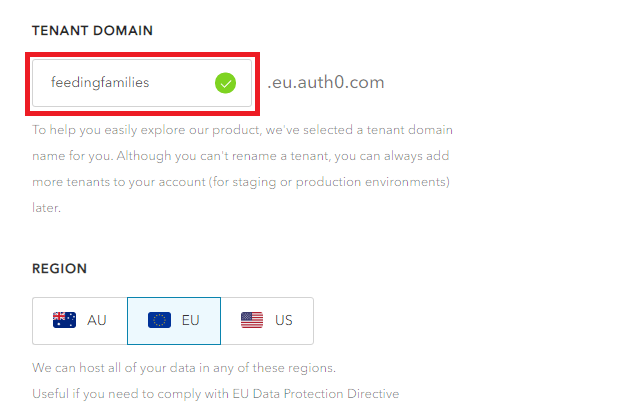
\includegraphics[width=0.8\textwidth]{auth0/tenantdomain.png}
\end{figure}
\noindent
Choose a fitting domain name for the authentication service to run on. This domain name is not the domain the volunteer portal will be accessed through, only the authentication service. Select the EU region to ensure quick access to the authentication service as all clients will be in the UK.\\

\noindent
After this screen you will need to select the plan that best suits you. We believe the free plan will be good enough to suit your needs but you can choose a different option, and if your needs increase in the future you can change the plan you're on at any point.\\

\noindent
You may also want to change a few settings. This can be done by clicking on the top right drop-down arrow.
\begin{figure}[H]
    \centering
    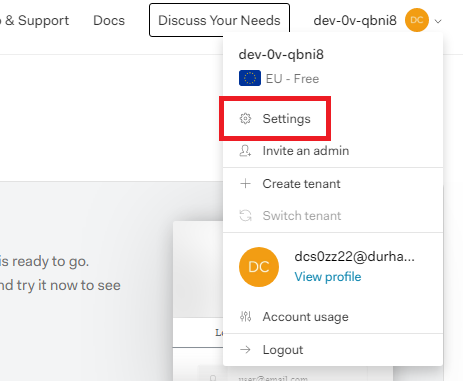
\includegraphics[width=0.8\textwidth]{auth0/settings.png}
\end{figure}
\noindent
Here you can add a 'friendly name', your logo, and support details. Here you can also change your subscription plan if you need to and allow other accounts access to your tenant domain and applications made with it.


\subsubsection{Creating an Auth0 application}
\begin{figure}[H]
    \centering
    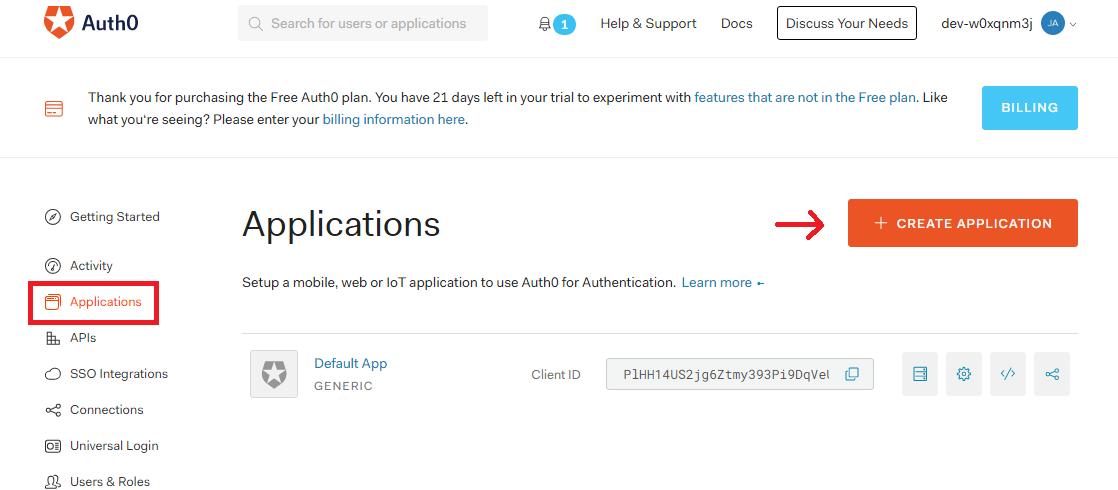
\includegraphics[width=0.8\textwidth]{auth0/application.png}
\end{figure}
\noindent
To set up the authentication service you need, click on the' applications' tab on the side bar, then the 'create application' button on the right. Then the following screen will appear.
\begin{figure}[H]
    \centering
    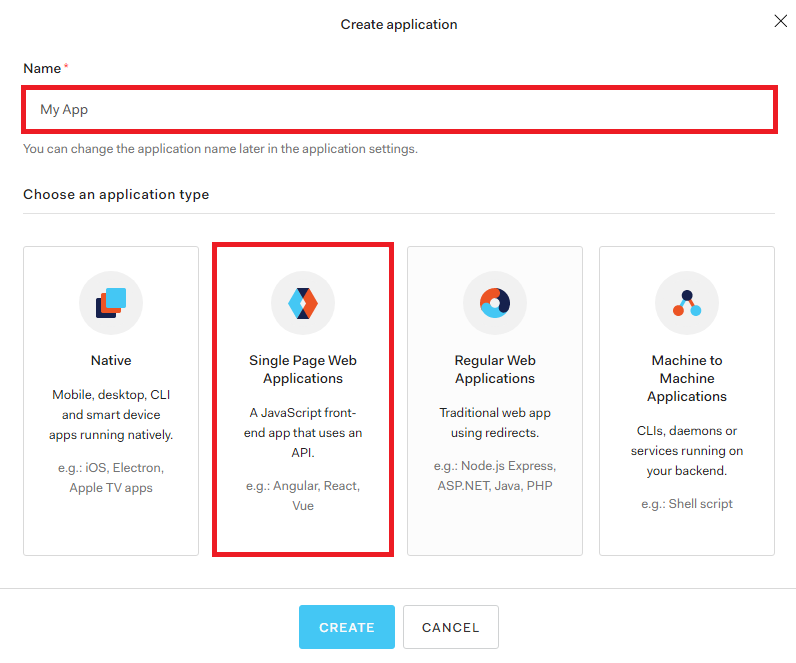
\includegraphics[width=0.8\textwidth]{auth0/createapp.png}
\end{figure}
\noindent
Set the name of the application, 'Feeding Families' is recommend but doesn't matter too much. It is important that the 'single page web applications' box is selected. Once the app is created, you will be taken to a quickstart page. You can      access the settings with the settings tab located below the application name.\\

\noindent
On the settings screen you need to set the URL the Feeding Families volunteer portal will be hosted.
\begin{figure}[H]
    \centering
    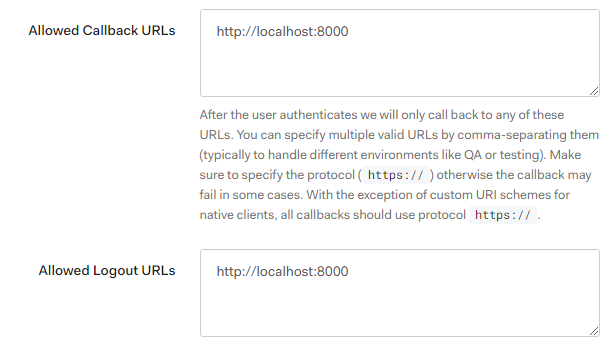
\includegraphics[width=0.8\textwidth]{auth0/urls.png}
\end{figure}
\noindent
Both the allowed callback URLs and Allowed Logout URLs need to be set. These will make sure login requests are only coming from people using your website. Note that the protocol is included (the http:// part of the URL). This should be https:// when the server hosting the volunteer portal is properly setup, as it will be secured. Also, the port number is included, that is the :8000. If the server is running on standard ports for the protocol, this can be omitted. For http that is 80 and https that is 443.\\

\noindent
Now you just need to create an API on Auth0, this is very simple. Start by clicking on 'APIs' on the sidebar.
\begin{figure}[H]
    \centering
    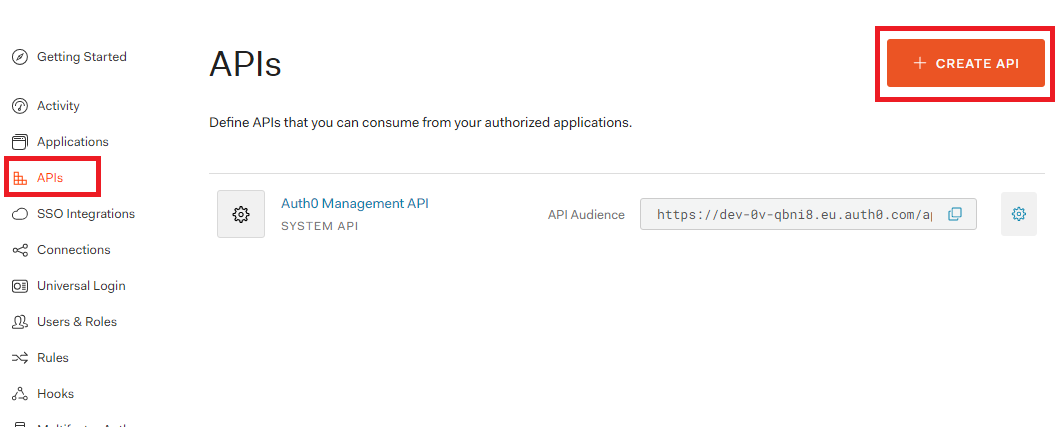
\includegraphics[width=0.8\textwidth]{auth0/Apis.png}
\end{figure}
\noindent
Then click the create API button. A screen like this will appear.
\begin{figure}[H]
    \centering
    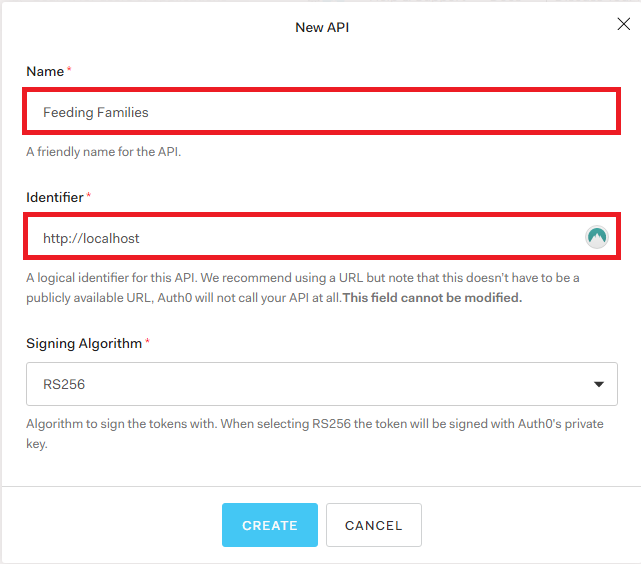
\includegraphics[width=0.8\textwidth]{auth0/newAPI.png}
\end{figure}
Give the API a name, this doesn't matter too much, and an identifier. This is important, it needs to be the URL the volunteer portal is hosted on and includes the protocol (http://).

\subsubsection{Linking to Auth0}
The last step is to link the volunteer portal to the auth0 service. All you need to do to achieve this is change a config file. The config file is in the client folder called \textbf{auth\_config.json}. When the file is open it should look like this: 
\begin{figure}[H]
    \centering
    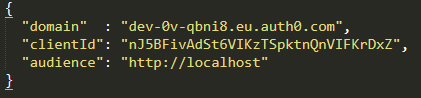
\includegraphics[width=0.8\textwidth]{auth0/config.png}
\end{figure}
\noindent
You must set the 'domain', 'clientId', and 'audience' parameters. To find the details you need to put there, go to the Auth0 application page and select the settings tab. The details are under the basic information header
\begin{figure}[H]
    \centering
    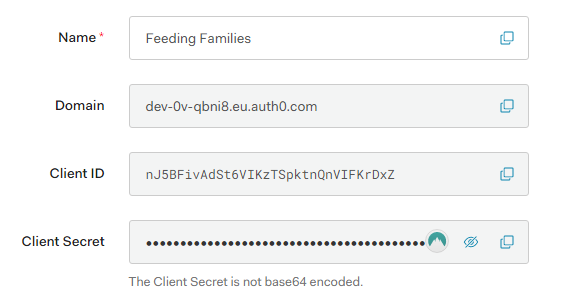
\includegraphics[width=0.8\textwidth]{auth0/configsettings.png}
\end{figure}
\noindent
Copy the domain and the client id from the auth0 page into auth\_config.json ensuring the quote marks surround the copied in domain and client id. Lastly the audience needs to be set, this is just the URL the volunteer portal is hosted on. In this case it is hosted locally so 'http://localhost' is used but if it hosted somewhere else enter that URL in. This needs to match the API audience on the Auth0 dashboard.


\newpage
\subsection{Server Setup}

\subsubsection{Installing the database}
The volunteer portal uses a mySQL database to hold the data, so you must have access to a mySQL server. This can be one hosted online or you can run the server on your local machine. An easy to setup mySQL server is \href{https://www.apachefriends.org/index.html}{XAMPP}. It also comes with a webserver which can be used to access the phpmyadmin portal to easily manage your database.\\

\noindent
Simply download and install \href{https://www.apachefriends.org/index.html}{XAMPP}. Once installed it should look like this:
\begin{figure}[H]
    \centering
    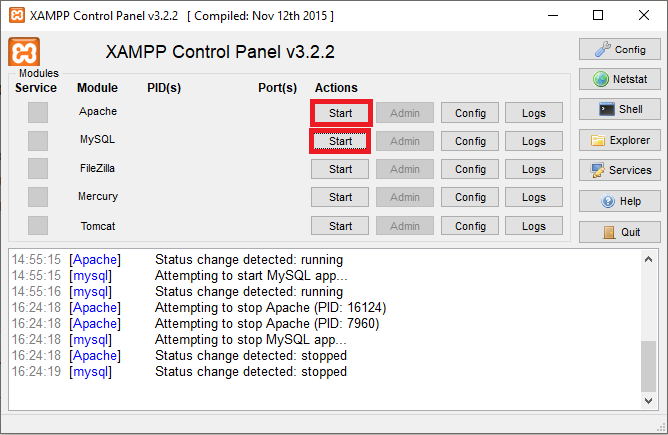
\includegraphics[width=0.8\textwidth]{serversetup/start.png}
\end{figure}
\noindent
Just click the start button for the Apache module and the mySQL module and you have a database server hosted on your local machine. \\

\noindent
Then you can click on the 'Admin' button for the mySQL module. You will be asked to sign in, the default admin account is 'root' with no password. When you are signed in you can change the password and this is recommended.\\

\noindent
 The next part is to create a database. Click the 'New' button on the left and name the database.
\begin{figure}[H]
    \centering
    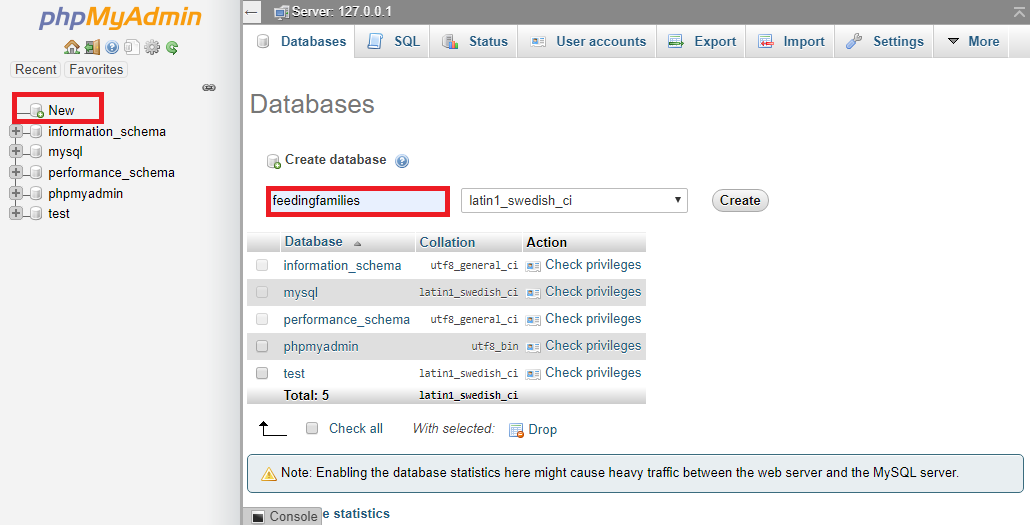
\includegraphics[width=1\textwidth]{serversetup/admincreate.png}
\end{figure}
\noindent
Then click the create button and your database will show up on the left. The screen will say there are no tables; the volunteer portal server will create the tables needed.\\

\noindent
Make sure the mySQL module is running when you want to start the volunteer portal server, the Apache module doesn't need to run, it is only to access the phpmyadmin tool.


\subsubsection{Installing the server}
The server runs on Node.js and so this must be installed on your system to be able to run it. To install, go to \href{https://nodejs.org/en/}{nodejs.org} and download the version for your computer.

\noindent
Once you have node installed on your system, you only have to navigate to the server files on your computer and open a terminal. On windows this can be done by typing in 'cmd' where the file path is.
\begin{figure}[H]
    \centering
    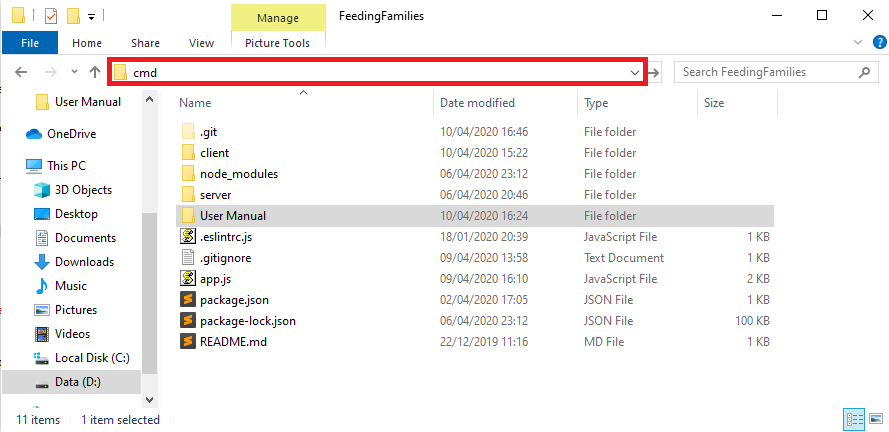
\includegraphics[width=0.8\textwidth]{serversetup/files.png}
\end{figure}
\begin{figure}[H]
    \centering
    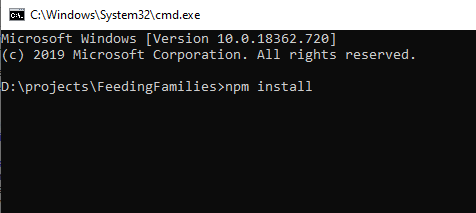
\includegraphics[width=0.8\textwidth]{serversetup/cmd.png}
\end{figure}
\noindent
Then, if node is properly installed, you just need to type the command 'npm install'. This will create the necessary files for the server. After the server is installed, run 'npm audit --fix' in the terminal to resolve any vulnerability issues due to outdated packages.\\

\noindent
To finish setting up the server, you need to tell it where the database is hosted. To do this go into the server folder and open 'config.json'
\begin{figure}[H]
    \centering
    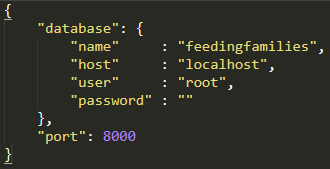
\includegraphics[width=0.8\textwidth]{serversetup/config.png}
\end{figure}
\noindent
The 'name' is the database name you set when creating the database. The 'host' is where the database is hosted, in this case it is local, so the host is localhost, if it is somewhere else provide the url of the database location. The 'user' and 'password' are the username and password to access the database. You can also change the port number the server is running on.\\
\noindent
Make sure to surround any values you add in quotation marks like shown.\\

\noindent
Now the server is ready to run, in the terminal you have open type: 'npm start' and the server will be running. Open your browser and go to localhost:8000 (the :8000 is the port number, change it if you changed the port) any you will be able to access the volunteer portal.

\newpage
\subsection{Cloud Deployment}
\subsubsection{Hosting Options}

For online deployment, there are two options:

\begin{itemize}
   \item Use Feeding Families' preexisting hosting package; or
   \item Use a separate cloud option:
   \begin{itemize}
        \item \href{https://www.hostinger.co.uk/}{https://www.hostinger.co.uk/}
            \begin{itemize}
                \item Good for small-medium businesses
                \item Provides weekly backups
                \item Cheap plan includes a database
            \end{itemize}
        \item \href{https://www.000webhost.com/}{https://www.000webhost.com/}
            \begin{itemize}
                \item Good for small businesses
                \item Easy to upgrade package
                \item Customer support
            \end{itemize}
   \end{itemize}
\end{itemize}

The pre-existing package may only be used if it can support a mySQL database storage option, as well as an additional website application. The separate cloud options all have multiple plans and even the cheapest options have minimum requirements for the hosting.

\newpage
\subsubsection{Deployment}
\href{https://www.heroku.com/}{Heroku} will be the service used to host the server in this demonstration and \href{https://remotemysql.com/}{remotesql} to host the database.\\

\noindent
\textbf{Remotesql}\\
\noindent
Setup an account on https://remotemysql.com/ you will have to confirm your account on email before continuing. Then click on the 'databases' tab on the sidebar then click 'create new database'
\begin{figure}[H]
    \centering
    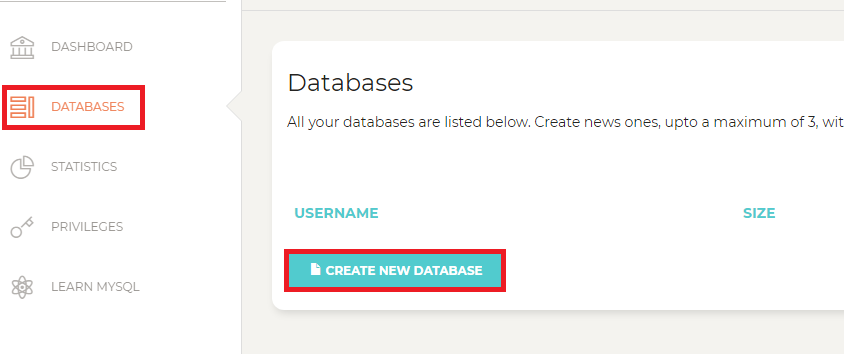
\includegraphics[width=0.8\textwidth]{deploy/databasecreate.png}
\end{figure}
\begin{figure}[H]
    \centering
    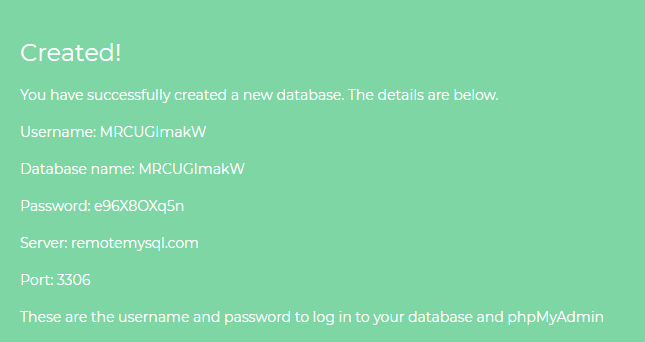
\includegraphics[width=0.8\textwidth]{deploy/created.png}
    \label{fig1}
\end{figure}
\noindent
These credentials will need to be used in the server config file. The host is 'remotesql.com', then the username. password, database name is as listed. Use the credentials you created for your account not the ones show in this manual.\\
\noindent
To view the database, you can use phpMyAdmin by clicking on the actions button next to the database.
\begin{figure}[H]
    \centering
    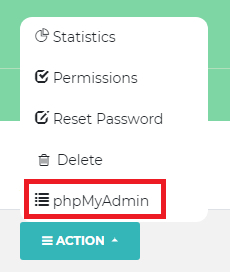
\includegraphics[width=0.5\textwidth]{deploy/admin.png}
\end{figure}
\noindent
This will allow you easily access the database and make changes if you want. This can make creating the initial admin user account easier.\\ 

\noindent
\textbf{Heroku}\\
\noindent
This requires your sever files to be on Github.\\

\noindent
Setup and account on \href{https://www.heroku.com/}{https://www.heroku.com/} you will need to verify your email to set up the account. Then click on 'create new app'. The next screen has the app name and region. The app name you choose will be in the domain 'appname.herokuapps.com', select the region to be in Europe. Then click 'create app', you will be taken to the deploy screen.
\begin{figure}[H]
    \centering
    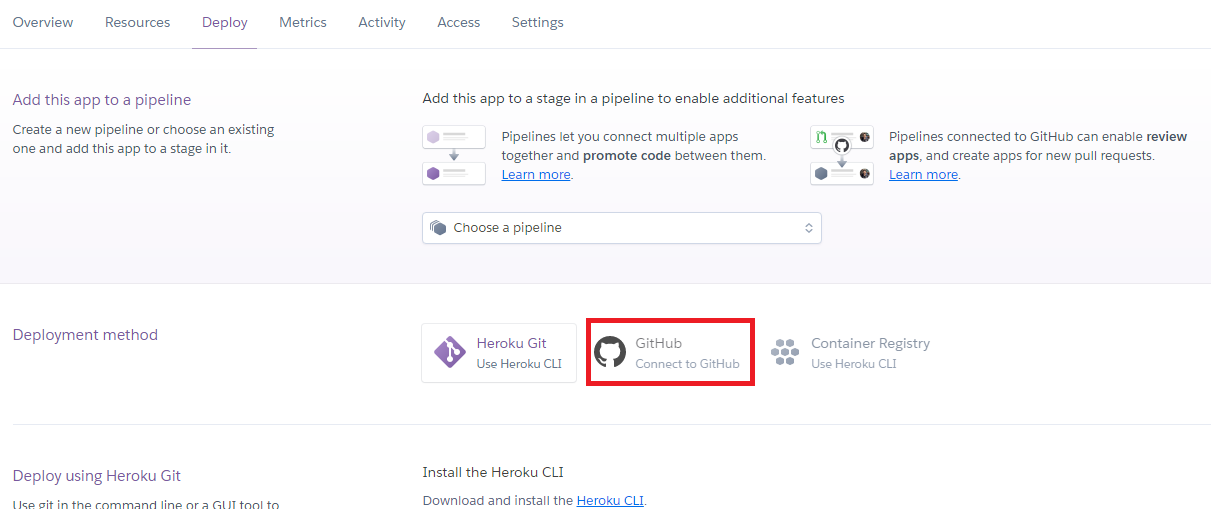
\includegraphics[width=1\textwidth]{deploy/deploy.png}
\end{figure}
\noindent
Click connect to GitHub and sign in. Then search for your repository where the server code is hosted and click 'connect'. Now you just have to click 'deploy branch' in the manual deploy section.
\begin{figure}[H]
    \centering
    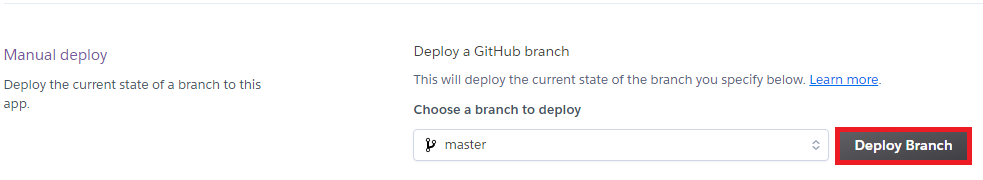
\includegraphics[width=1\textwidth]{deploy/manual.png}
\noindent
\end{figure}
\noindent
Just wait a while for the server to deploy, all the server set up will be done for you. Make sure you have set up the database config file before deploying or you will cause the server to crash on start and set up Auth0 and auth\textunderscore config.json for the URL the server is being hosted.
\begin{figure}[H]
    \centering
    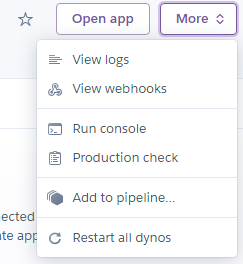
\includegraphics[width=0.5\textwidth]{deploy/openapp.png}
\end{figure}
\noindent
Finally, you can open the website by clicking 'open app' at the top-right or view the logs of the server by clicking 'more> view logs'. The logs can be helpful to see if the server has launched correctly and to identify any errors.


\subsubsection{Hosted Demonstration}
A demonstration of the system is hosted at \href{https://feedingfamilies.herokuapp.com/}{https://feedingfamilies.herokuapp.com/}. It has some dummy data on it so you try it out from a volunteers point of view, or as an admin and try out the functions of the admin panel. The admin account's login details are \textbf{email: dcs0zz22@durham.ac.uk, password: FeedingFamilies1}

\newpage
\section{Getting Started} %%%%%%%%%%%%%%%%%%%%%%%%%%%%%%%%%%%%%% Section 3

\subsection{Login Page}

The login page is the first component of the feeding families volunteering portal. Users are able to click the ‘sign in’ button which redirects them to an Auth0 website. 

\begin{figure}[h]
    \centering
    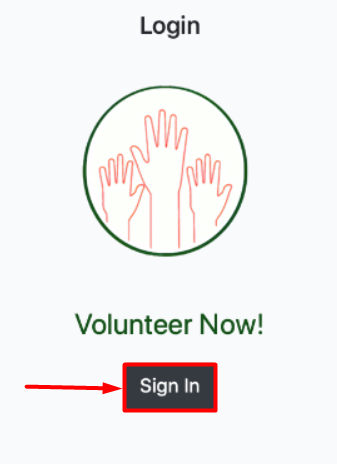
\includegraphics[width=0.5\textwidth]{main/login.png}
    \caption{Login Redirect Subsection}
    \label{fig1}
\end{figure}

Auth0 is our method of adding authentication and authorization services to our application. Each time a user tries to authenticate, Auth0 will verify their identity and send the required information back to the application. 
\newpage

The portal has a header which lists the relevant areas to the volunteering process, as well as providing an easy method of returning back to the feeding families home page, with the 'home' button.

\begin{figure}[h]
    \centering
    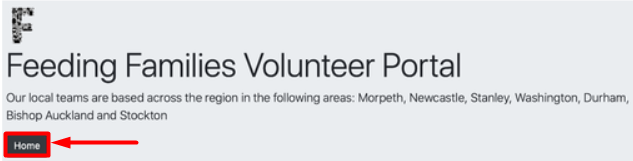
\includegraphics[scale=0.8]{main/rsz_portaltitle.png}
    \caption{Portal Title}
    \label{fig2}
\end{figure}

Feeding Families' social links can also be accessed from the main login page by clicking on the appropriate image in the details subsection of the portal.

\begin{figure}[h]
    \centering
    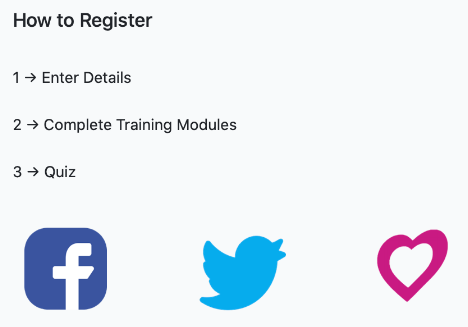
\includegraphics[scale=0.9]{main/registerlinks.png}
    \caption{Portal Details Subsection}
    \label{fig3}
\end{figure}
\newpage
\vspace{1.0cm}

\subsection{Logging In}

Upon clicking the login button, the user is redirected to a page which looks like the figures shown below. Here they can login using their existing google account as shown in Figure~\ref{fig4a}, or they must create a new account if they do not own one by switching to the sign up tab as shown in Figure~\ref{fig4b}.

\begin{figure}[h]
 
    \begin{subfigure}{0.515\textwidth}
    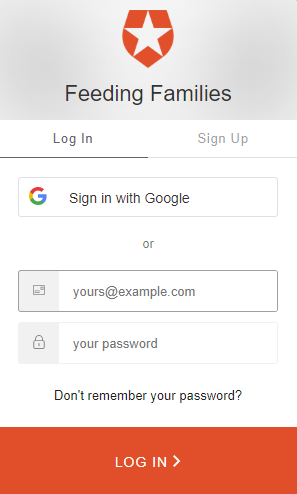
\includegraphics[width=0.9\linewidth]{main/loginredirect1.png} 
    \caption{The log-in window.}
    \label{fig4a}
    \end{subfigure}
    \begin{subfigure}{0.5\textwidth}
    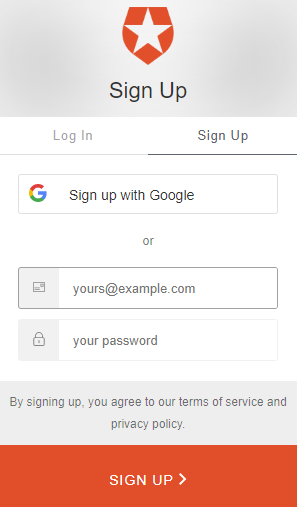
\includegraphics[width=0.9\linewidth]{main/loginredirect2.png}
    \caption{The register window.}
    \label{fig4b}
    \end{subfigure}
 
\caption{Login screens.}
\label{fig4}
\end{figure}

Upon successfully logging in, the main website will be accessed instantly via redirect.
\newpage

\section{Volunteering Forms} %%%%%%%%%%%%%%%%%%%%%%%%%%%%%%%%%%%%%% Section 4
\subsection{Choosing volunteer type}

Users should now see the following page:

\begin{figure}[h]
    \centering
    \hspace*{-2cm}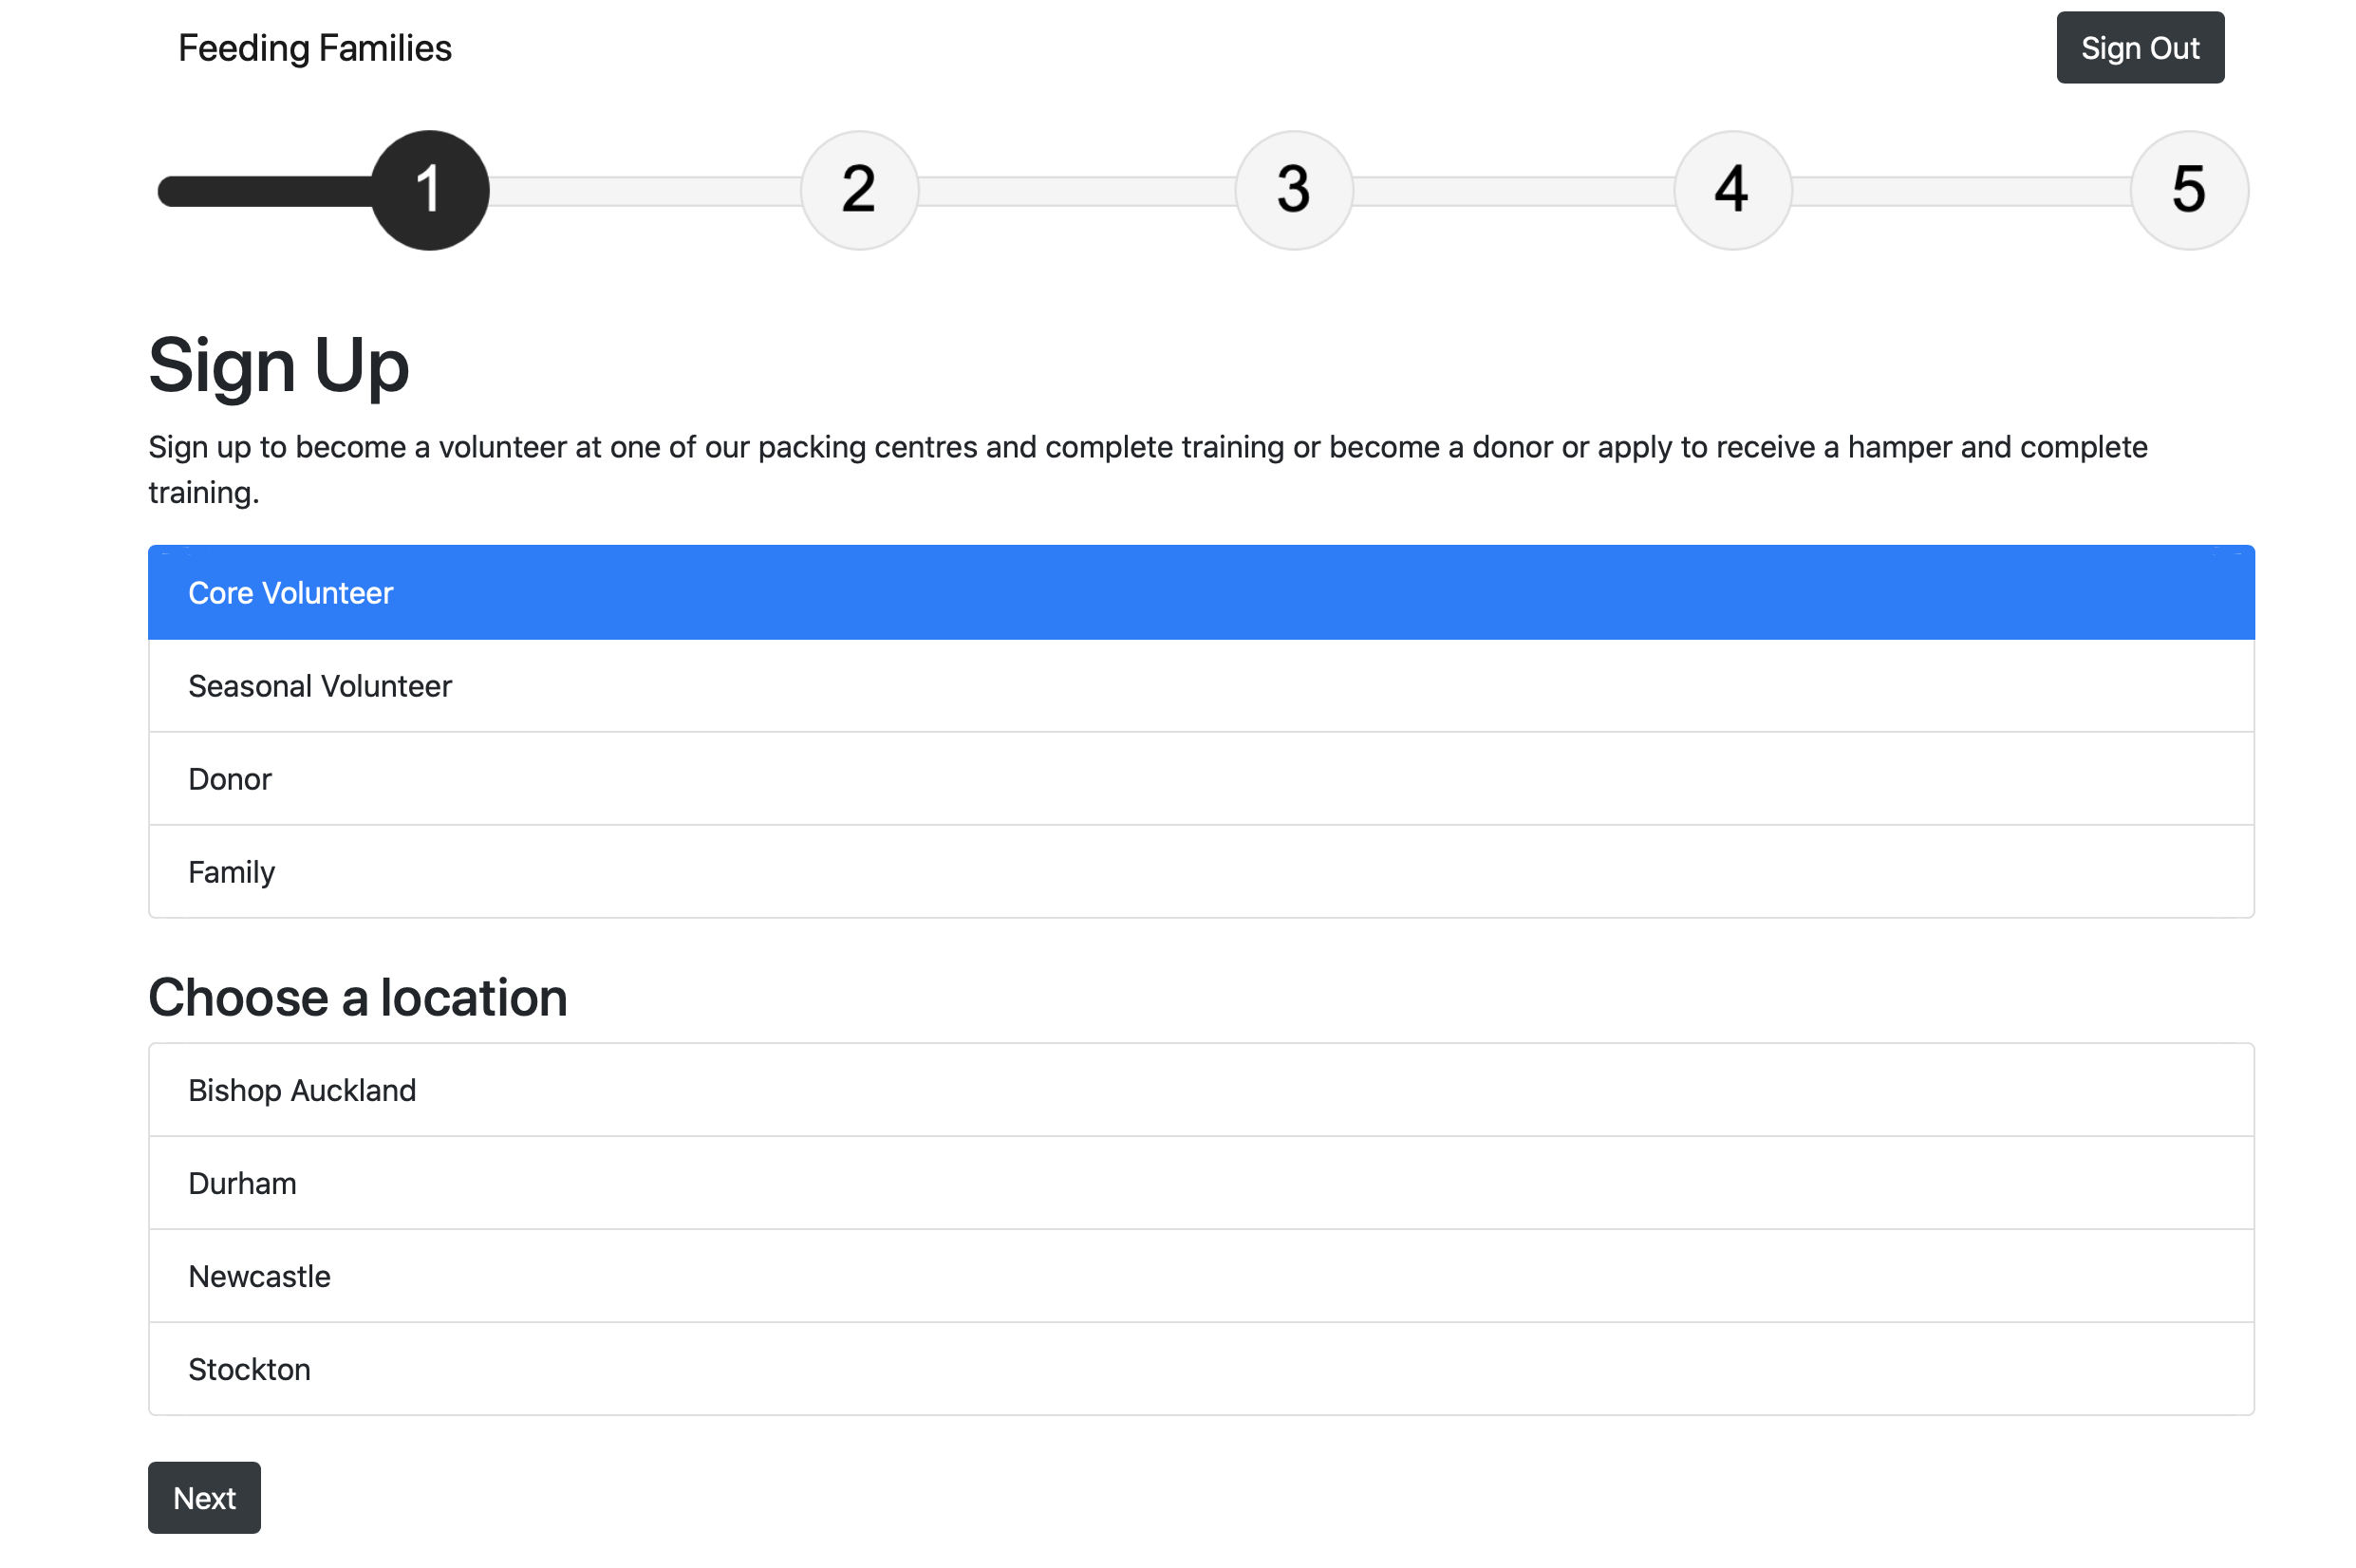
\includegraphics[scale=0.3]{main/main.png}
    \caption{Main volunteering page}
    \label{fig5}
\end{figure}

There are multiple conditional options, such as the locations and the 'Seasonal Volunteer' option, which are only available as and when the admin sets them to be active. The user must select one from four options followed by an accompanying location:

\begin{itemize}
   \item Core volunteer 
    \item Seasonal volunteer 
   \item Donor (Donate hampers); or
   \item Family (Receiving hampers).
   
\end{itemize}

\newpage
\subsection{Donor and Family Forms}
Both the Donor and Family options require the user to submit the same personal data. The form is as shown in Figure~\ref{fig6}.

\begin{figure}[h]
    \centering
    \hspace*{-2cm}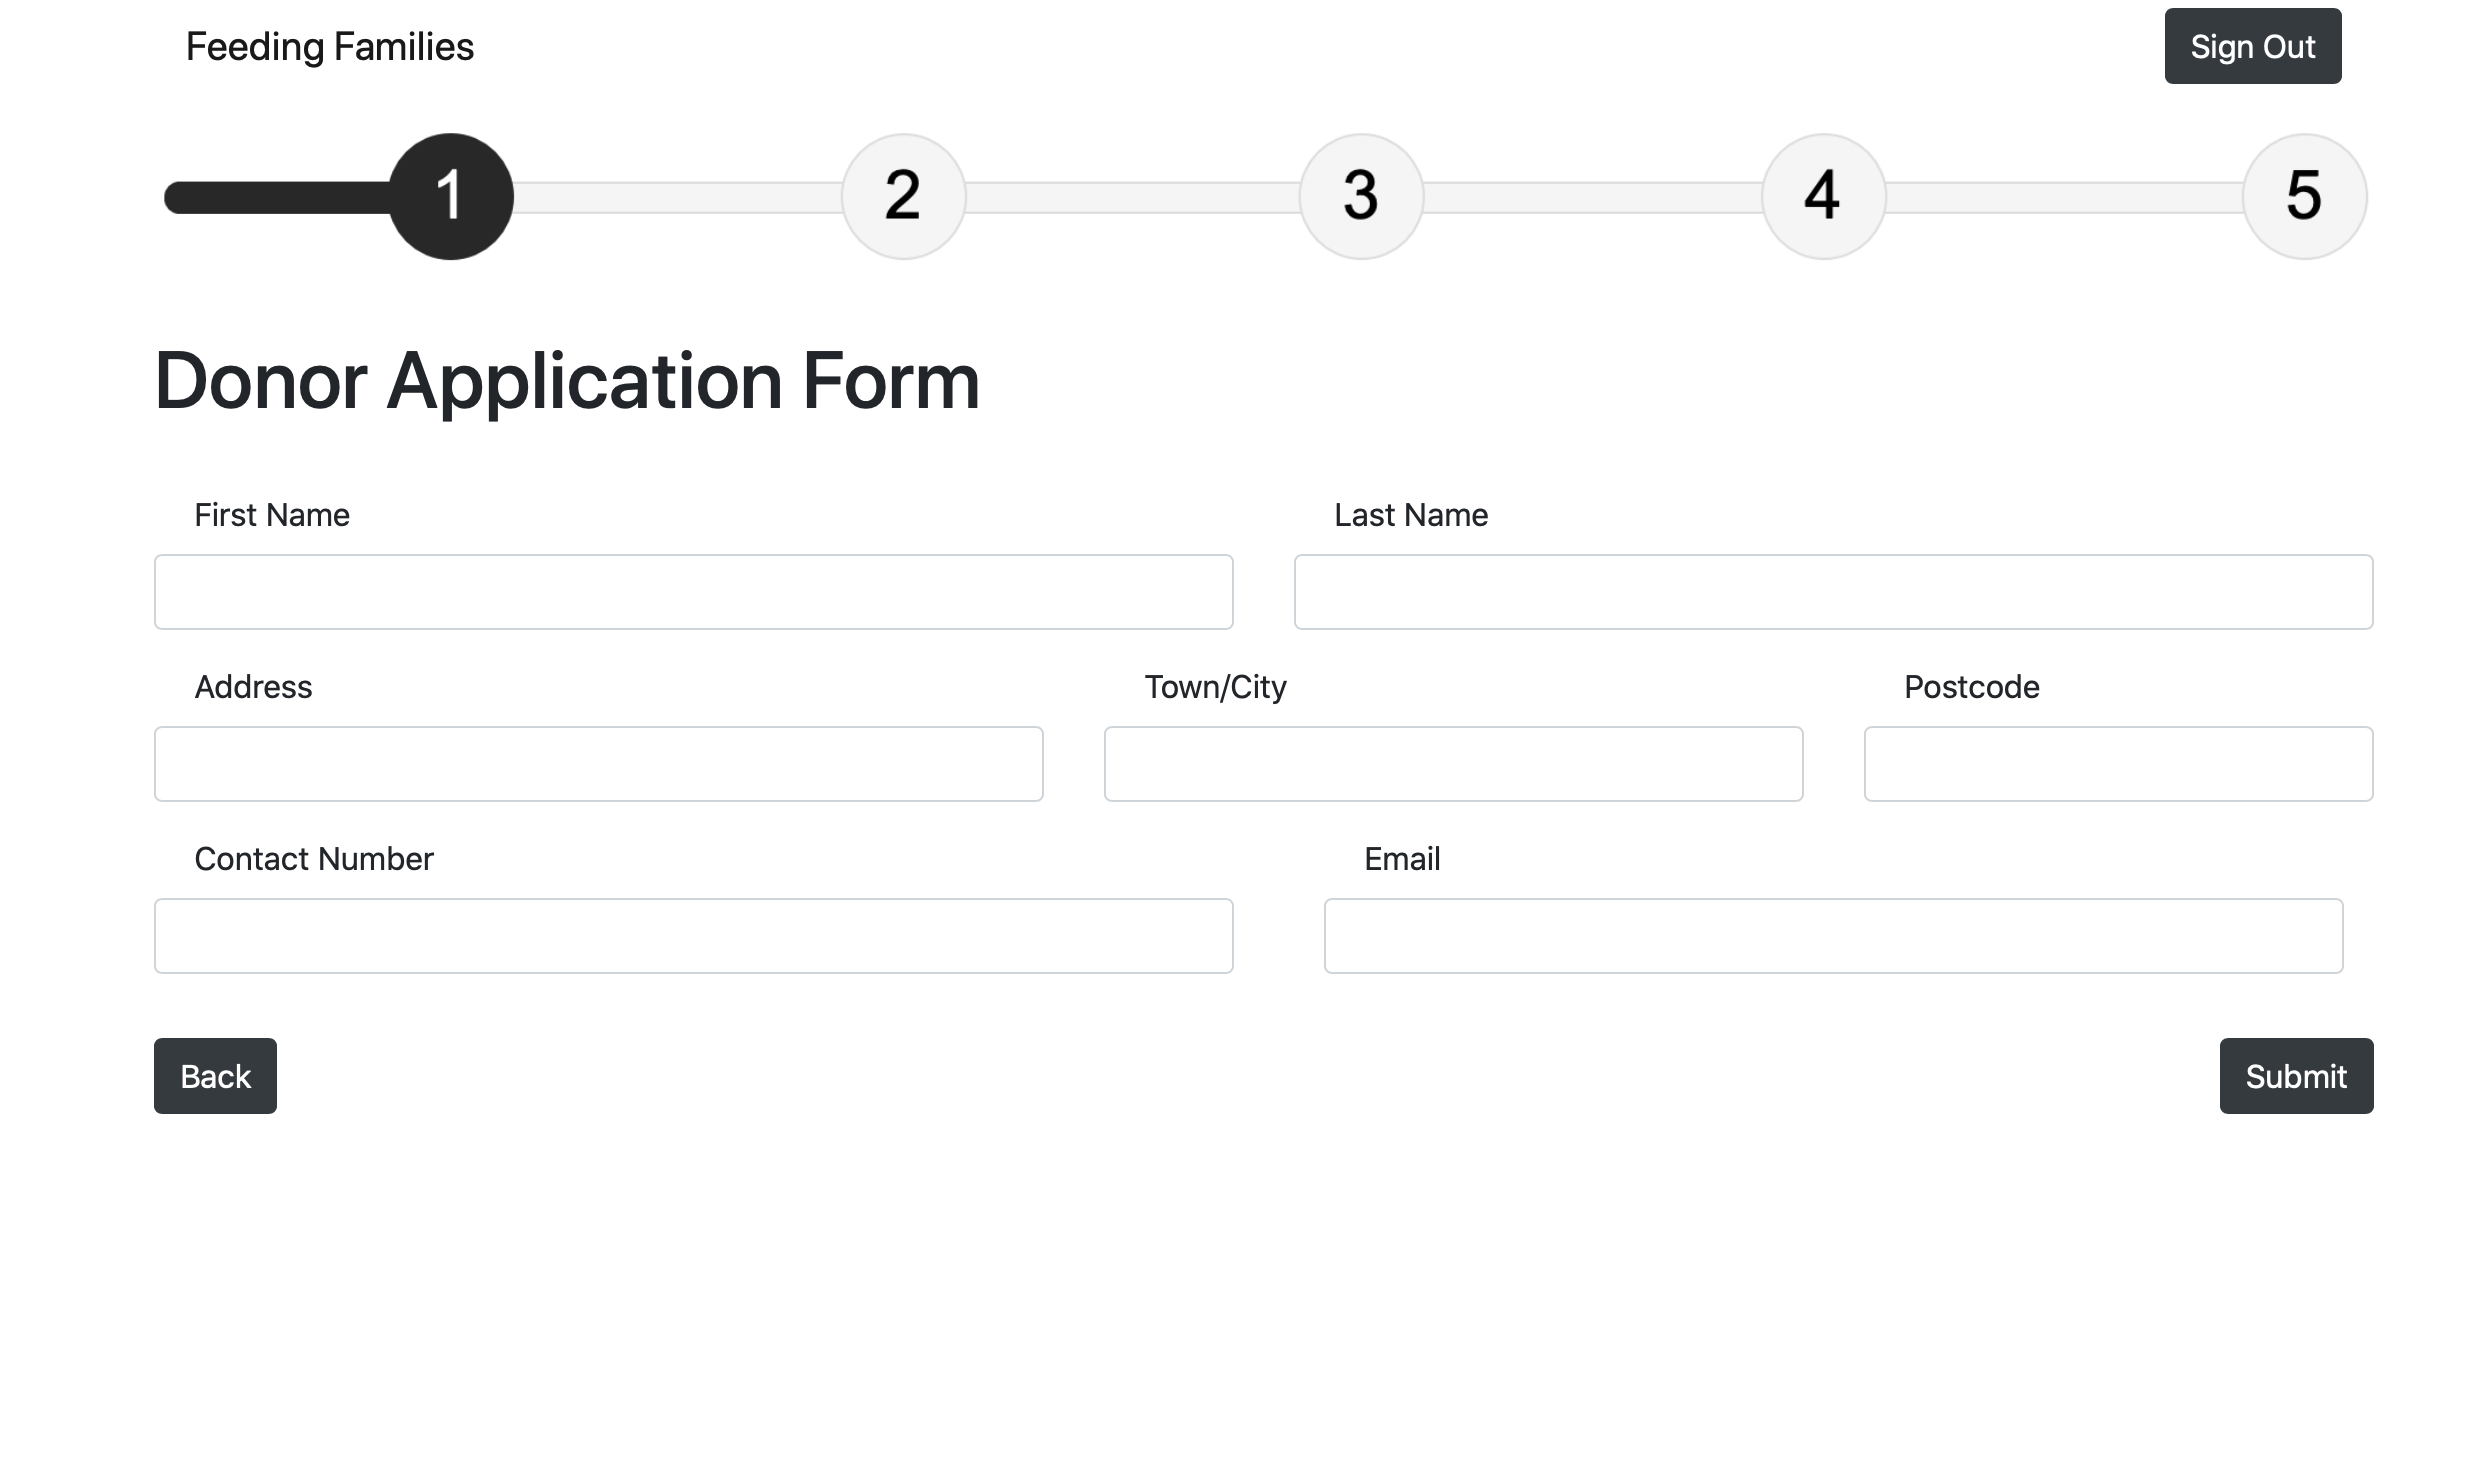
\includegraphics[scale=0.4]{main/donor.png}
    \caption{Donor page}
    \label{fig6}
\end{figure}

The user may return to the main volunteering page if their form was chosen incorrectly (Figure~\ref{fig7a}). However, if chosen correctly and \textbf{all} forms are filled, the user can submit their information (Figure~\ref{fig7b}), which will bring them to the training modules section of the sign-up process. 
\begin{figure}[h]
 
    \begin{subfigure}{0.515\textwidth}
    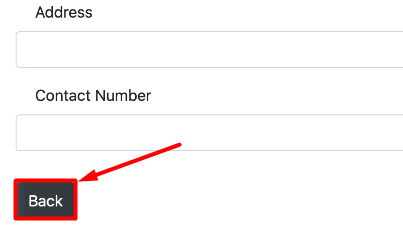
\includegraphics[width=0.9\linewidth]{main/Back.png} 
    \caption{Return from form.}
    \label{fig7a}
    \end{subfigure}
    \begin{subfigure}{0.5\textwidth}
    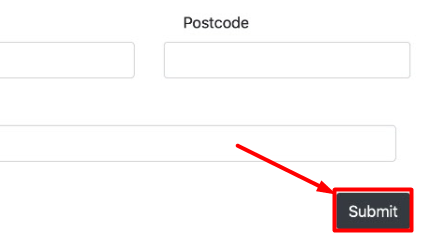
\includegraphics[width=0.9\linewidth]{main/submit.png}
    \caption{'Submit' to continue.}
    \label{fig7b}
    \end{subfigure}
 
\caption{Form navigation}
\label{fig7}
\end{figure}
\newpage
Furthermore, the user can log out and exit at any time by using the log out button provided in the top right of the page and each subsequent page to follow:

\begin{figure}[h]
    \centering
    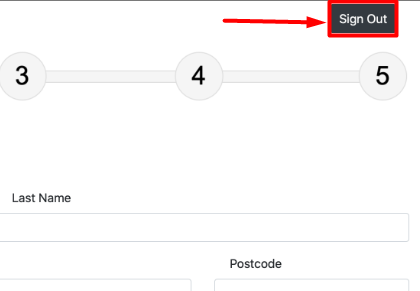
\includegraphics{main/signout.png}
    \caption{Sign out}
    \label{fig8}
\end{figure}
\newpage

\subsection{Seasonal Form}
\begin{figure}[h]
    \centering
    \hspace*{-2cm}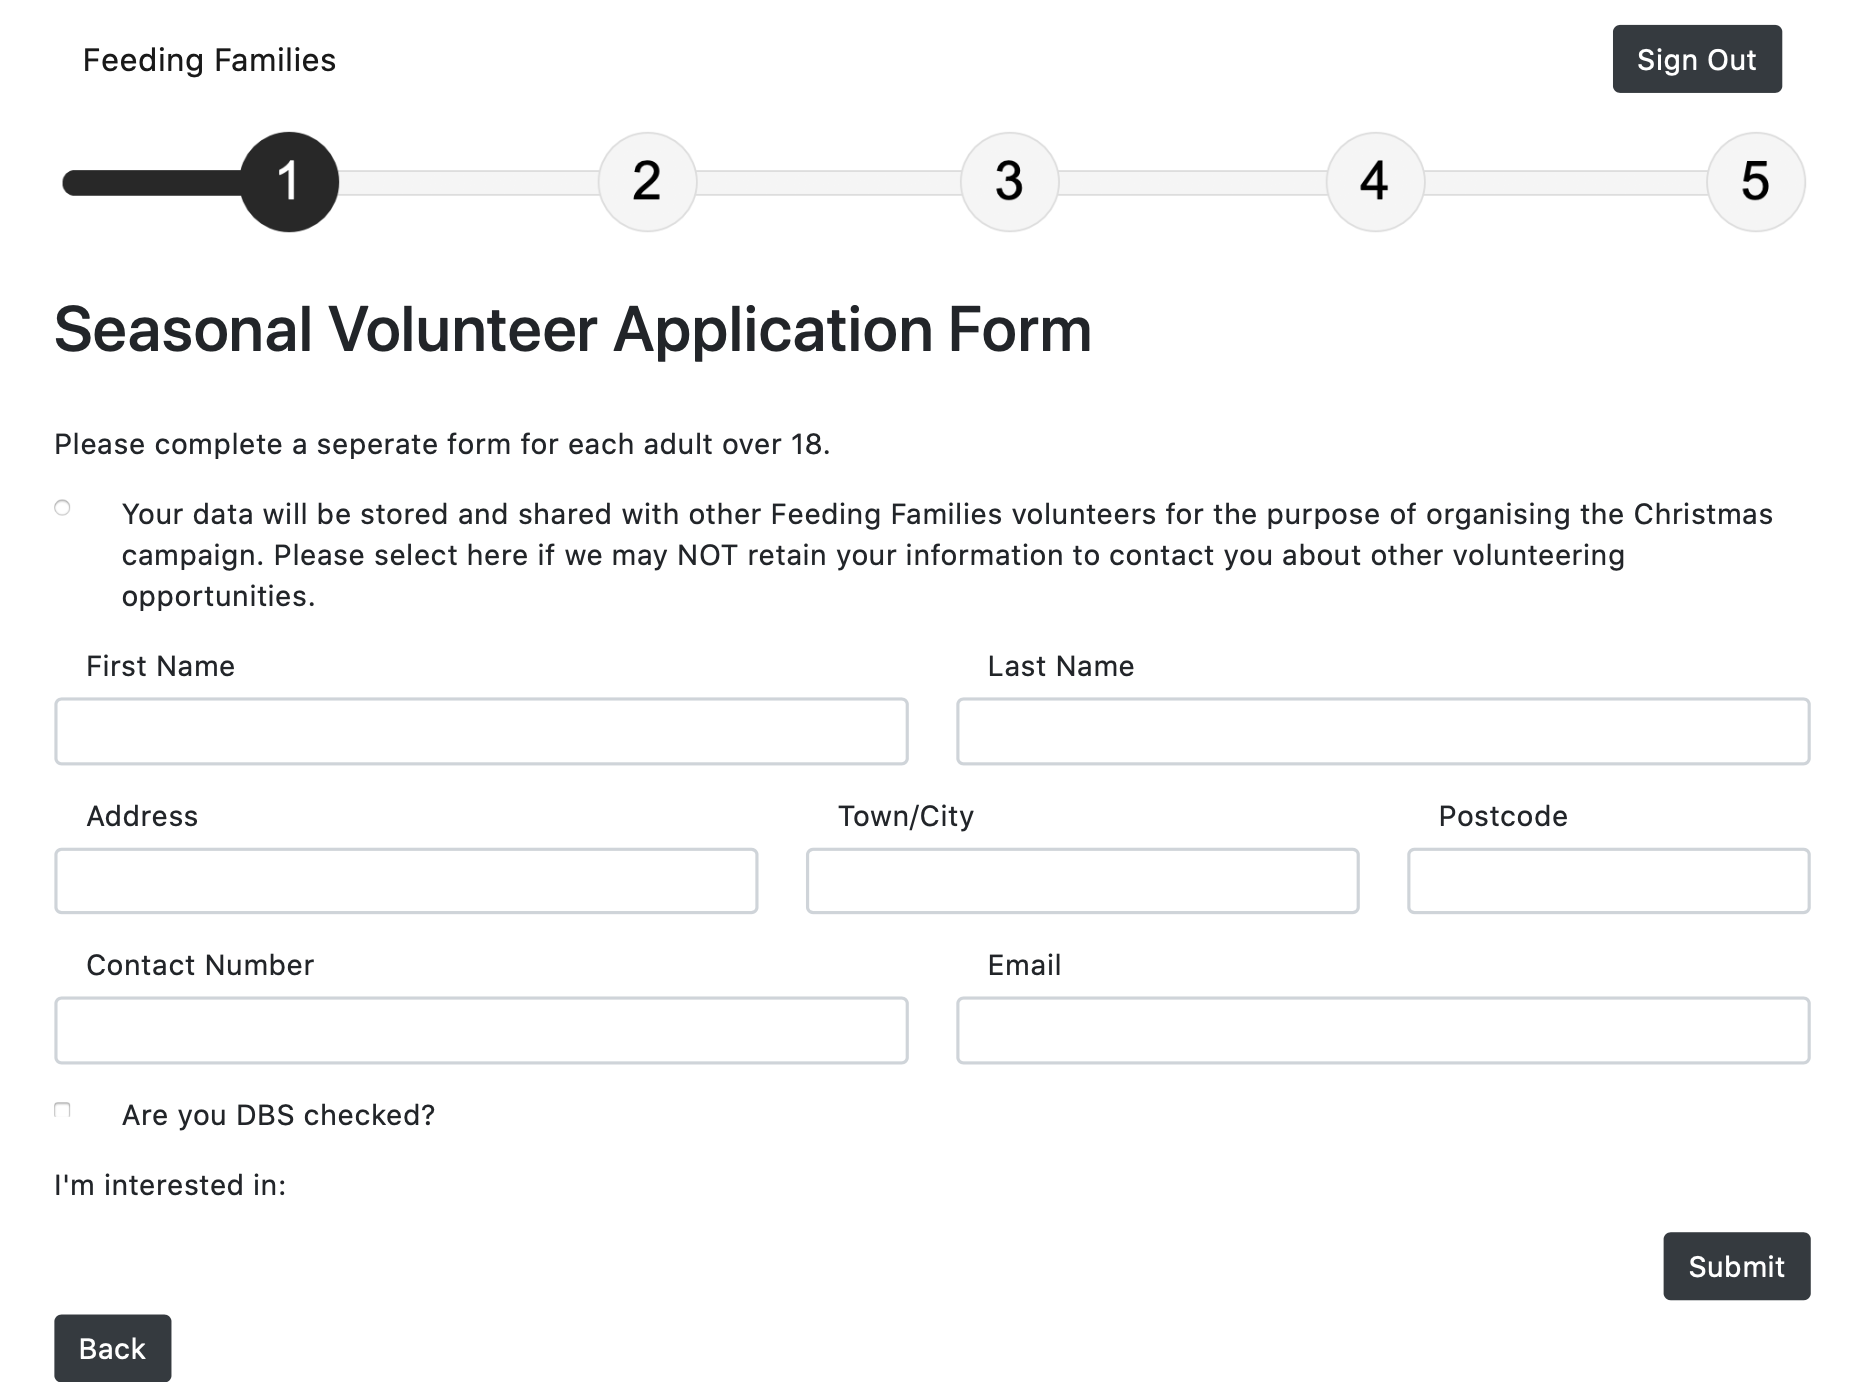
\includegraphics[scale=0.4]{main/seasonal.png}
    \caption{Seasonal page}
    \label{fig9}
\end{figure}

The seasonal form is similar to the donor/family forms, however the applicant should agree to the storing and sharing of their data with the other volunteers involved with feeding families, state that they are DBS checked (which is a requirement) and select their dates of choice.

\newpage
\subsection{Core Form}

\begin{figure}[h]
    \centering
    \hspace*{-2cm}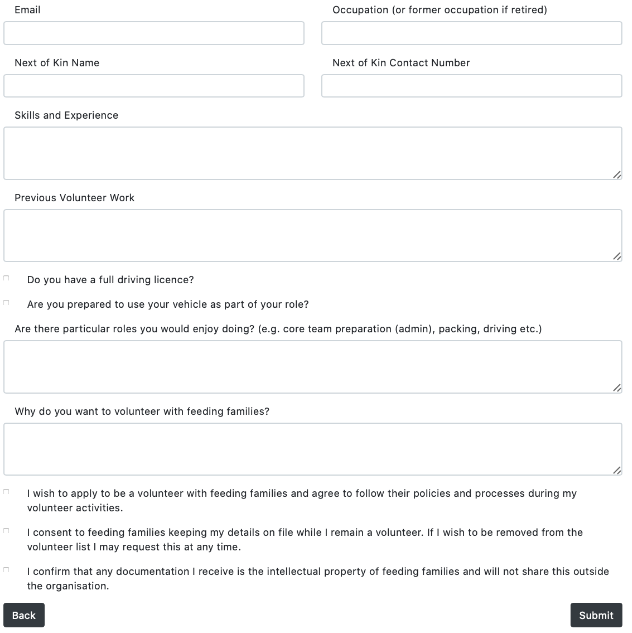
\includegraphics[scale=0.8]{main/coreadditions.png}
    \caption{Core page}
    \label{fig10}
\end{figure}

The core form requires all of the information provided in the seasonal form and some additional data, since they are more involved with the project. They must also agree and consent to the conditions provided at the bottom of the page in order to move onto the training modules.
\newpage
\section{Admin Access} %%%%%%%%%%%%%%%%%%%%%%%%%%%%%%%%%%%%%% Section 5

\subsection{Creating Admin Accounts}
To create an admin account you need database access, this is so other admins cannot add or remove people from being add, only someone who controls the system should be able to do and the persons with database access already have access to all the data so they should be the ones to create admin accounts.\\
\noindent
This is only for admin accounts with the most privileges, manager accounts can be added easily through the admin panel.\\ 

\noindent
To add an admin account, access your database. In this guide we are using phpMyAdmin to have an easy graphical interface with the database. 
\begin{figure}[H]
    \centering
    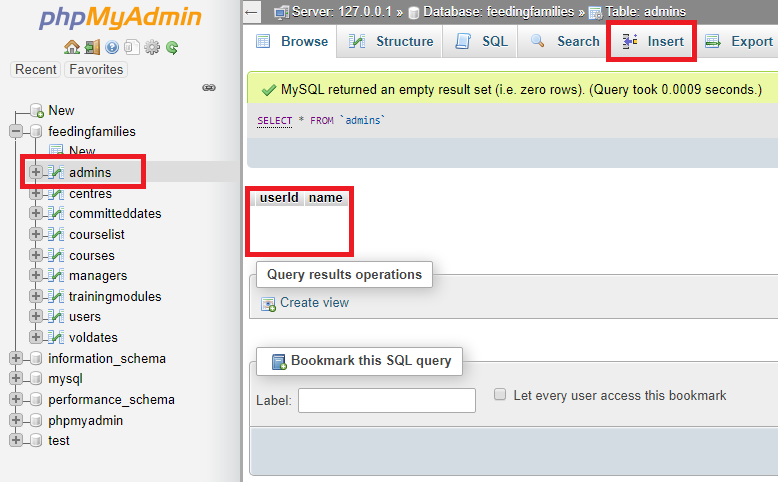
\includegraphics[width=1\textwidth]{admins/table.png}
\end{figure}
\noindent
Find the admins table in your database in the sidebar and click it. The screen will show all the current admin userIds and name, at the moment there aren't any admins, so the table is empty. Then click insert.
\begin{figure}[H]
    \centering
    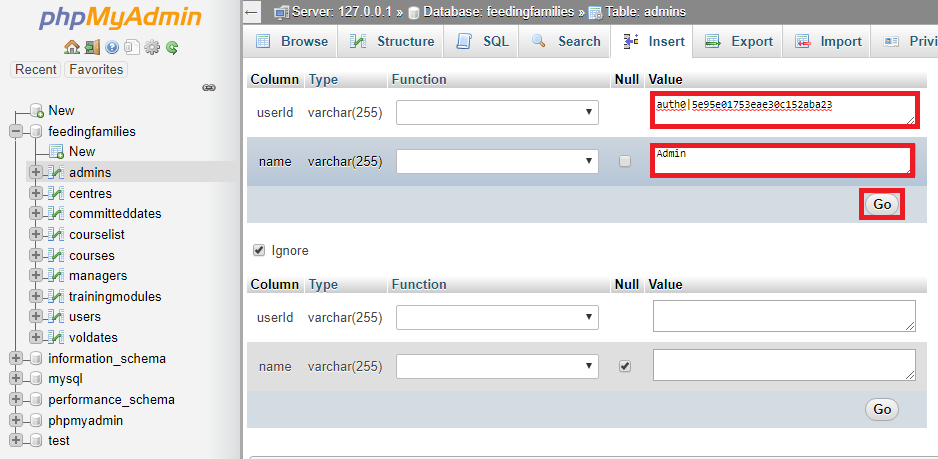
\includegraphics[width=1\textwidth]{admins/insert.png}
\end{figure}
\noindent
Enter the user's id you want to be admin, then their name (the name doesn't matter it's just so you can keep track of who is who). Then that data will be inserted, and you can see that by clicking on the admins table on the sidebar again or by clicking the 'browse' tab at the top.\\

\noindent
\textbf{Getting the user id}\\
\noindent
The user id is generated by Auth0 and is used in the users table to identify users. In order to create your first admin account, you need to get your userId, this can be done by simply filling out one of the volunteer forms and submitting it so your userId can be found in the users table.
\begin{figure}[H]
    \centering
    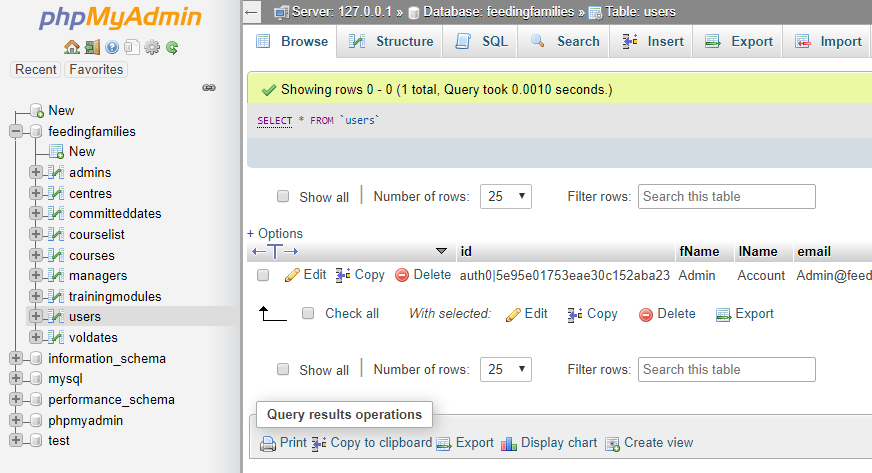
\includegraphics[width=1\textwidth]{admins/users.png}
\end{figure}
This is after logging in with Auth0 on the account you want to make an admin and filling in a core volunteer form. You can now copy the id from this table and use it to create the admin account. you can then delete this entry in the users tables as it is not necessary.\\

\noindent
The second way to get your user id is to sign in with your account, then open the browser console. This can be done with inspect element, then select the console tab at the top.
\begin{figure}[H]
    \centering
    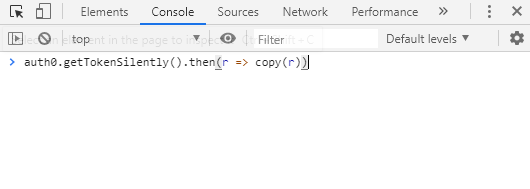
\includegraphics[width=0.6\textwidth]{admins/console.png}
\end{figure}
\noindent
Then enter the command \lstinline"auth0.getTokenSilently().then(r => copy(r))", this will copy your access token to your clipboard. Now go to \href{https://jwt.io/}{jwt.io} and paste in to the left side box labelled 'encoded'. 
\begin{figure}[H]
    \centering
    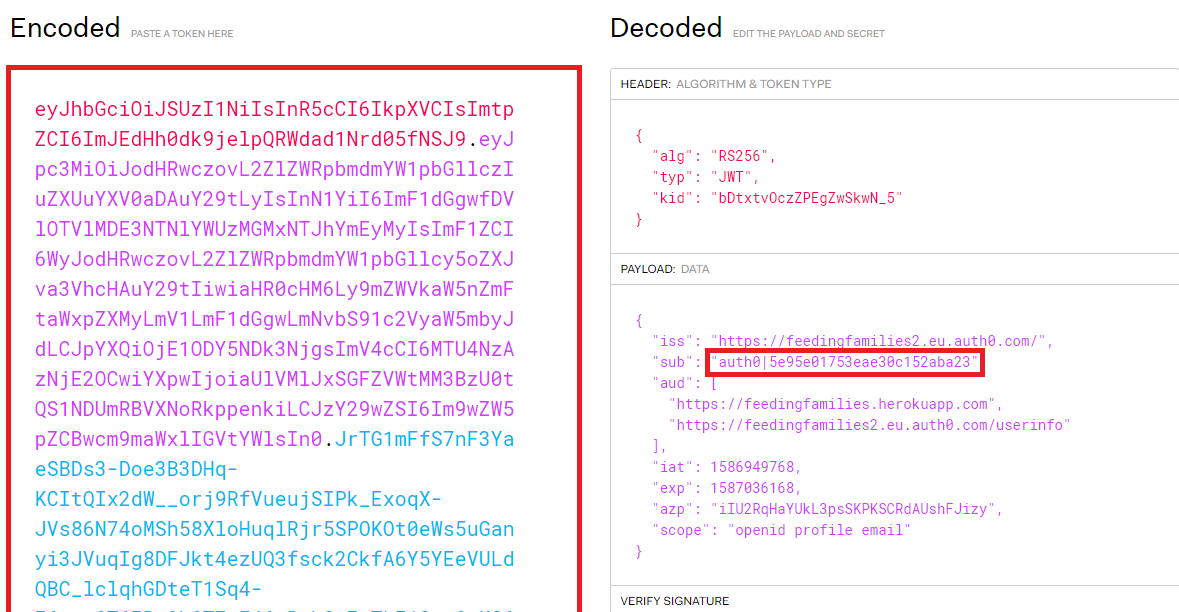
\includegraphics[width=1\textwidth]{admins/jwt.png}
\end{figure}
\noindent
The user id is listed on the right in the 'payload' section, it is the variable 'sub'. Copy the id without the quote marks then you can use it to insert and admin account.\\

\noindent
Once you have one admin account it is easier to find user's ids using the admin panel. You can use the user search function and click the button to expose the user's id, then you can add that to the admin table through the database.
\newpage
\subsection{Admin Accounts}
Once you have access to an admin account, you will be able to log in to see the following screen, from which you can continue to access the admin dashboard;

\begin{figure}[H]
    \centering
    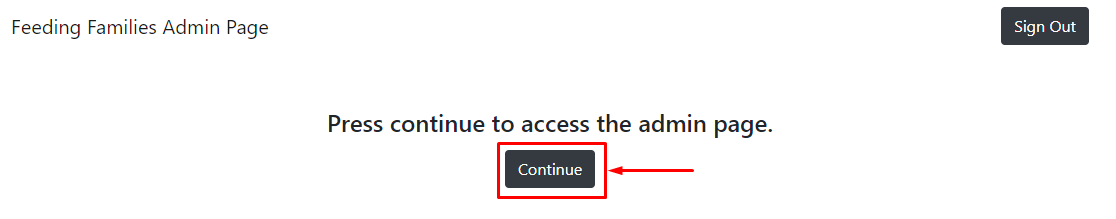
\includegraphics[width=1\textwidth]{admins/adminaccess.png}
\end{figure}

Next, you have access to a variety of different tools which you can utilize:
\begin{itemize}
   \item Amending Seasonal Dates
   \item Searching for Users
   \item Amending Managers
   \item Amending Centres
   \item Exporting stored data into CSV files
   
\end{itemize}

\begin{figure}[H]
    \centering
    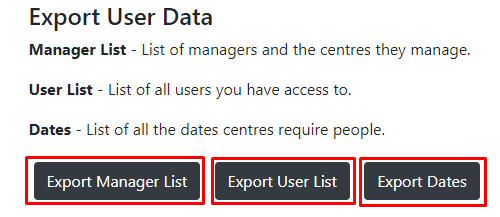
\includegraphics[width=1\textwidth]{admins/export.png}
    \caption{Exporting user data - Admins can collect CSV files for excel use.}
\end{figure}


\begin{figure}[H]
    \centering
    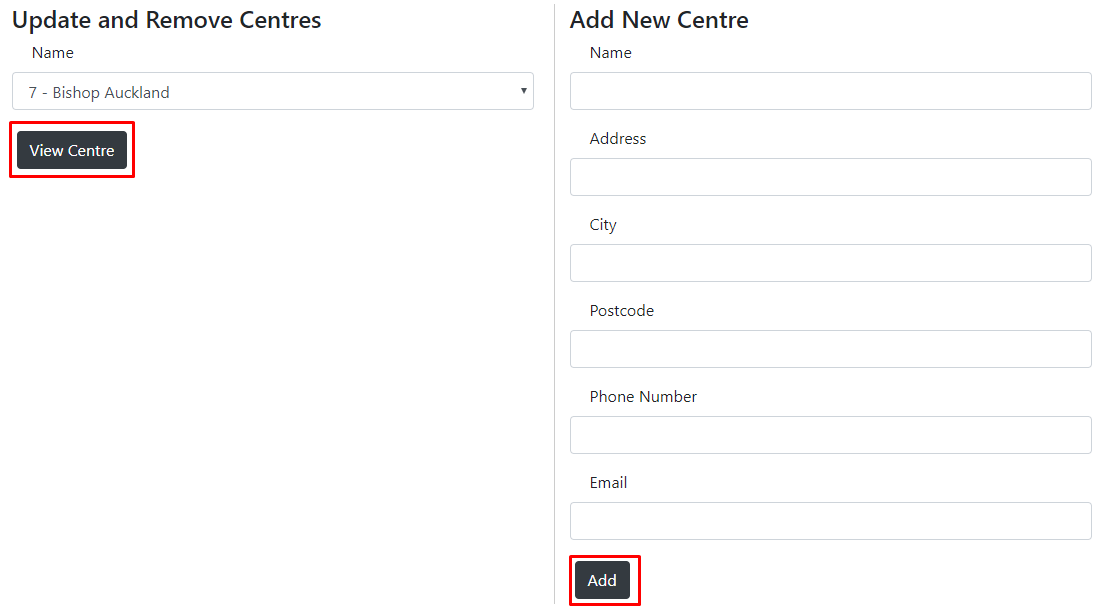
\includegraphics[width=0.9\textwidth]{admins/centres.png}
    \caption{Amending Centres - Admins can add or remove centres as they please.}
\end{figure}

\begin{figure}[H]
    \centering
    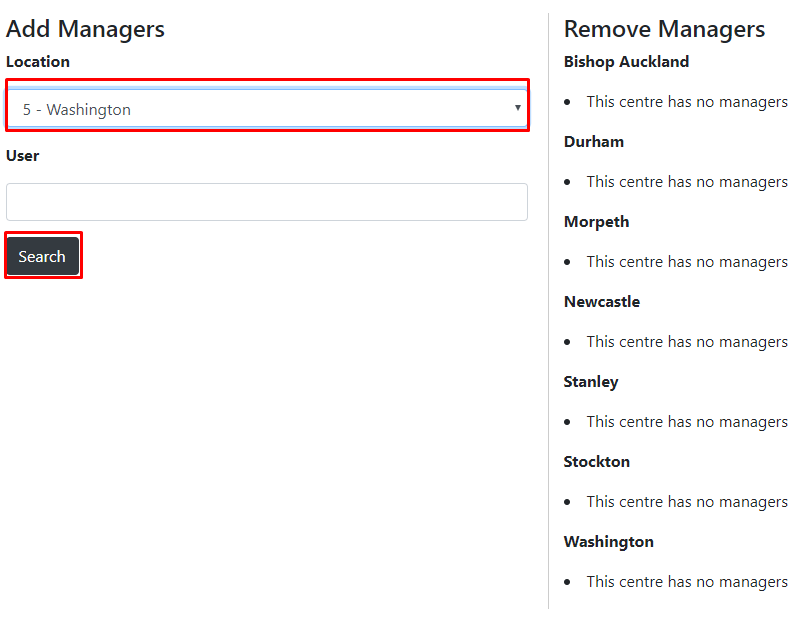
\includegraphics[width=0.8\textwidth]{admins/addmanagers.png}
    \caption{Amending Managers - Admins can add or remove Managers as they please.}
\end{figure}
\newpage

\begin{figure}[H]
    \centering
    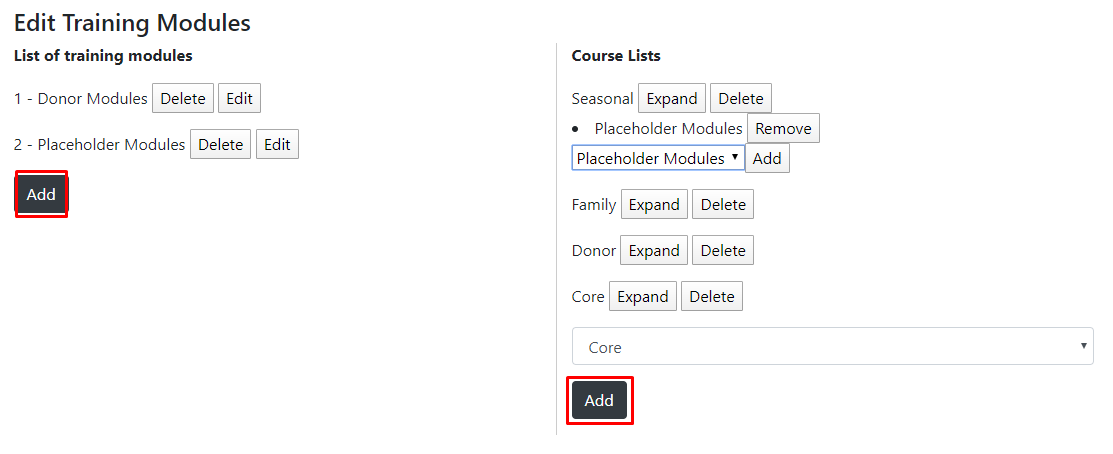
\includegraphics[scale=0.7]{admins/Training Modules.png}
    \caption{Amending Managers - Admins can add or remove Training Modules.}
\end{figure}

The admin dashboard is very flexible and has all the features required to update the application as and when required. It makes the collection of the Auth0 ID for any user trivial, so that new users can be converted in admins should Feeding Families wish to do so. 
\newpage
\section{API} %%%%%%%%%%%%%%%%%%%%%%%%%%%%%%%%%%%%%% Section 6

\subsection{Making Authenticated Requests}
Many of the API endpoints are authenticated to ensure a request is coming from a valid user and they have permission to access that endpoint. To use these endpoints, you must set an authorization header in your requests.

\noindent
The first thing you need to do is get your JavaScript Web Token(JWT) which will be used to authenticate your request. To get this token you just have to access the variable 'auth0', this has the async function 'getTokenSilently'. The user must be signed in at this point.
\vspace{0.5cm}
\begin{lstlisting}
auth0.getTokenSilently()
.then(token => doSomething);
\end{lstlisting}
\vspace{0.5cm}
\noindent
Once you have the token, this is valid for 10 hours (can be changed on your Auth0 account) or until the user signs out, you can use the token to make authenticated requests like so
\vspace{0.5cm}
\begin{lstlisting}
fetch("/api/admins/check",
	{
		method: "GET",
		headers: {
			"Authorization": `Bearer ${token}`
		},
	})
.then(response => response.json())
.then(data => doSomething);
\end{lstlisting}
\vspace{0.5cm}
\noindent
The API will handle all your permissions and send back the response, that's all that is needed to make requests to the authenticated endpoints of the API.


\subsection{Endpoints}
All the endpoints of the API are documented in the 'server/endpoints/docs' folder, they are split into multiple files based on their function to make it easier to find the endpoints you need. The structure of the documentation is as follows:\\
\noindent
\begin{itemize}
\item The Endpoint route followed by the request type (GET or POST) and 'Authenticated' if it requests authentication.
\item A description of what the endpoint does.
\item A list of encoded variables, if it is a post request the variables will go in the body of the request, if it is a get request the variables will be encoded in the URL. URL encoded variables will be stated in the endpoint route with a colon preceding them, for example '/api/admins/user/search/:name' name is the encoded variable and should be replaced as so '/api/admins/user/search/Alice'
\item The response in JSON format, when the data type is plural it indicates the data will be list of that datatype. 

\end{itemize}

\noindent\\
\textbf{documentation for all the endpoints can be found in the ‘server/endpoints/docs’ folder}

\newpage

\section{System Maintenance}
\subsection{Database}

\subsubsection{Design}
The database is written in MySQL accessed via the Node.js module 'mysql' (\href{https://www.npmjs.com/package/mysql}{https://www.npmjs.com/package/mysql}). All the code that access the database directly can be found in the \textbf{server/db} folder.\\

\noindent
\textbf{connection.js}\\
\noindent
This is a very simple file and only establishes the connection to the database server for all subsequent files to use. All the database connection information is stored in the \textbf{server/config.json} file to centralise server configuration.\\

\noindent
\textbf{create.js}\\
\noindent
This file is responsible for creating all the tables in the database. SQL queries occur asynchronously and since this database uses foreign keys, some tables rely on other tables existing before this table can be created. This file uses promises and then chains to make sure the tables are created in a specific order each time.\\
If at any time an error occurs in creating the tables, the system throws the error and crashes out - without properly setting up tables, the system cannot continue.\\


\newpage
\noindent
\textbf{generic files}\\
\noindent
All other files are named after the table they make queries to. All the SQL code is in the form:
\begin{lstlisting}
function foo(variable, ...) {
	return new Promise((resolve, reject) => {
		sql.connection.query("SELECT * \
		FROM table\
		WHERE id = ?", 
		[variable, ...], 
		function(error, results) {
			if(error) reject(error);
			else resolve(results);
		});
	});
}
\end{lstlisting}
The function wraps the \href{https://www.npmjs.com/package/mysql}{mysql} code in a promise to resolve the need for callback functions and instead can be handled with promise-then chains. 'sql.connection' comes from the connection.js file as connection is an export of that file, the query method on that connection is used to query the database it connects to. Note the use of the '?' and the list of variables as the second parameter of the query method, this is the way to create prepared statements with the \href{https://www.npmjs.com/package/mysql}{mysql} package and prevents SQL injection.\\

\noindent
Note also that the callback function can take two variables, the first is set if there is any error, and the second is any results. A query may not generate any results so this second variable can be left out.\\

\newpage
\noindent
\textbf{Database Relational Diagram}\\
\begin{figure}[H]
    \centering
    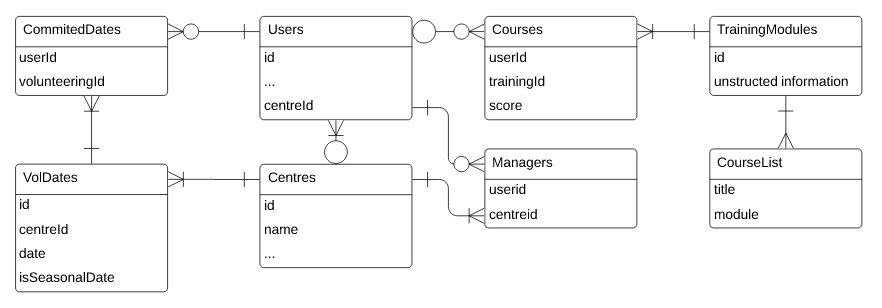
\includegraphics[width=1\textwidth]{design/database.png}
\end{figure}
\noindent
This database is in 3\textsuperscript{rd} normal form. This is useful to avoid data duplication and maintain relational integrity. It makes writing SQL queries for specific data easy and simple and no processing to collate data needs to be done in JavaScript this way.\\

\noindent
\textbf{Users}\\
The users table holds all the users of the system and all the data about those uses. The unstructured field of this table is for any unstructured data you need to hold on this user. For a core volunteer, this will hold information about why they want to volunteer, if they have a driving license, and other information collected in the sign-up form. The centreId is the id of the centre they volunteer are and this links to the centres table.\\

\noindent
\textbf{Centres}\\
The centres table holds information about the centres Feeding Families operate. Each entry of the table has a unique ID and important contact information for this centre is also stored.\\

\noindent
\textbf{Managers}\\
This table is used to identify user with elevated privileges. For each centre a user manages, their userId will be stored with that centreId. This table keeps the database in normal, instead of storing managers of a centre in the 'centres' table; this is important to maintain relational integrity.\\

\noindent
\textbf{VolDates}\\
This is the volunteering dates table and it holds the data about dates volunteers are needed. The date is linked to a centre as not all the centres will have people doing things on the same dates. The description field is used to for a bit of information on what volunteers will be doing, for example 'packing'. The capacity is the maximum number of volunteers that can sign up to that date.\\

\noindent
\textbf{CommitedDates}\\
This table records userIds and the dateIds they have signup to. This table maintains the normal form and prevents data duplication.

\noindent
\textbf{TrainingModules}\\
This table holds all the module information, the important field of this table is the content or unstructed field. This field has the content and structure of the training module stored in JSON format.\\

\noindent
\textbf{Courses}\\
This table is here to keep the database in normal form and prevent data duplication. Each training module a user takes is stored as a separate entry.\\

\noindent
\textbf{CourseList}\\
This table sets out what modules a user will need to take depending on how they signup. The title is used in the system to get the correct modules for the user. For example: if a user signs up as a core volunteer they will enrol on the courselist 'core'.\\

\subsubsection{Development}
For further developments, it is recommended you read the design section as it details how most queries are formatted. The database code is written in Node.js using the mysql package (\href{https://www.npmjs.com/package/mysql}{https://www.npmjs.com/package/mysql}).\\

\noindent
\textbf{Adding new tables}\\
All the tables are created in the create.js file. To add a new table add .then(() =\textgreater createYourTable) at the bottom of the then chain, before the catch. Example follows.
\newpage
\begin{lstlisting}
...
.then(() => {
	return new Promise((resolve) => {...})
})
.then(() => {
	return new Promise((resolve) => {
		mysql.connection.query("CREATE TABLE\
		IF NOT EXISTS table(...)",
		function(error) {
			if(error) throw error;
			resolve();
		});
	});
})
.catch(error => {throw error;});
\end{lstlisting}

\noindent
\textbf{Adding or changing queries}\\
The format for creating new queries can be found in the design section under the generic file header. Ensure that your functions are included in modules.exports so they can be accessed outside of the file. These functions can also do some processing on the data coming from the queries such as bit values being turned into Booleans for easy use. You can also do some processing on data before it goes into the database. If you wanted to add encryption to some fields of the tables, you could do the encryption and decryption inside these functions.\\ 

\noindent
\textbf{Changing database type}\\
If there is a need to change the database for scalability reasons or anything else, you just need to edit the functions keeping the names and their outputs the same as they currently are. Ensure that the functions still return promises as the API code uses promise-then chains.


\subsection{API}
\subsubsection{Design}
The server is run on Node.js and express (\href{https://expressjs.com/}{https://expressjs.com/}). The app.js file is the main server that serves the client and backend. The constant 'express' is exported so the endpoint files can access it and create endpoints.\\

\noindent
\textbf{Endpoints}\\
\noindent
All endpoints are separated into different files, so endpoints related to the same things are kept together, leading to easier navigation of the code. Most endpoints are fairly simple, consisting of some input validation and checks on the user, followed by a database operation then sending the results to the user. A generic endpoint looks as follows.

\begin{lstlisting}
app.app.post("/api/endpoint/", app.checkJwt, (req, resp) => {
	doSomething()
	.then(data => {
		return resp.status(200)
			.send({status: 200, data: data})
	})
	.catch(err)
})
\end{lstlisting}
app is app.js required which has the express constant app exported, so app.app just accesses the express constant. Then the request type is post. The first parameter is the endpoint you want to access this code. The second parameter is option, include this if you want this endpoint to be authenticated. Finally, the third is the function you want to run.

\subsubsection{Development}
\textbf{Creating a new file}\\
\noindent
If a new table has been created or you want to add functionality not closely related to the existing functionality you should create a new file. For this file to be used: at the top of the file has include:
\begin{lstlisting}
const app = require("../../app.js");
\end{lstlisting}
This points to the app.js in the root directory, if you have created your file in a different folder to the other endpoints you will need to make sure it points to the app.js file. Then in the app.js include a line that requires your file.
\begin{lstlisting}
//Endpoints
require("./server/endpoints/centres.js");
...
require("./server/endpoints/exports.js");
require(".server/endpoints/yourfile.js");
\end{lstlisting}
Now this file can be served when its endpoints are called.\\

\noindent
\textbf{Creating new endpoint}\\
\noindent
To create a new endpoint, first choose which file you want to create it, what is it most related to? Create a new file if it is very different. Creating a new endpoint is fairly simple just follow the generic endpoint in the design section. It is important to include the catch in case there is an error, the server will catch it and respond to it instead of crashing.\\
\noindent
\textbf{Encoded variables}\\
\noindent
For post requests: the encoded variables are in the body of the request so to access them use \lstinline"req.body" this is an object of all the variables set in the body of the request. For get request: you can have variables encoded in the URL or variables encoded as queries. The URL are set in \lstinline"req.params", to have express allow these variable, use a colon to denote a part of the URl as variable like so \lstinline"/api/foo/:variable/bar/", this will be accessed with \lstinline"req.params.variable". Query variables can be accessed with \lstinline"req.query".

\end{document}
